\documentclass{article}
\usepackage[utf8]{inputenc}
\usepackage[francais]{babel}
\usepackage[T1]{fontenc}
\usepackage{lmodern}
\usepackage{ifpdf}
\usepackage{pdflscape} % ou lscape
\usepackage{graphicx}
\renewcommand{\familydefault}{\sfdefault}

\title{Guidage des étudiants par GPS sur le Campus Triolet, UM2 - Android}
\author{PAGÈS Julien \and SALEIL Baptiste \and BENGHABRIT Walid}
\date{\today}
\ifpdf
	\pdfinfo 
	{
		/Author (Pagès - Saleil - Benghabrit)
		/Title (Guidage des étudiants par GPS sur le Campus Triolet, UM2 - Android)
		/Subject (Guidage des étudiants par GPS sur le Campus Triolet)
		/Keywords ()
		/CreationDate (\today)
	}
\fi

\begin{document}
	% Page de titre
	\maketitle
	\thispagestyle{empty}
	
	\newpage
	\tableofcontents
	
	\newpage
	\section{Introduction}
	Avec l'essor des plateformes mobiles aujourd'hui, le but premier du projet était de découvrir la plateforme Android et plus généralement être initié aux aspects des systèmes embarqués intelligents. \\
	le but du projet était de développer une application utilisant différents composants d'Android.
	C'est donc un projet dans un cadre universitaire, et nous avons choisi de faire un guidage des étudiants sur le campus, les deux aspects sont donc bien présents, une application universitaire et mobile, de plus cette application nous semble utile pour les nouveaux arrivants. \\
	Le but final est d'avoir une application fonctionnelle tout en sachant que nous découvrons la plateforme et qu'on ne pourra pas avoir un résultat comme celui qu'aurait une entreprise développant depuis plusieurs années sur Android. \\
	Nous sommes assez libres sur les fonctionnalités à implémenter, ainsi nous avons choisi d'avoir une application fonctionnelle qui utilise plusieurs composants du système et exploite les avantages de l'embarqué (GPS, données mobiles etc). \\
	
	\section{Cahier des charges}
	Cette section présente un petit cahier des charges.
	Il présente les fonctionnalités que nous souhaitions développer pour l'application, et une exemple des différentes vues disponibles.
	
	\subsection{Caractéristiques}
	\begin{itemize}
		\item Interface simple, rapide, intuitive \\
			Le but ici est de fournir la meilleure expérience possible a l'utilisateur. Tout doit être accessible rapidement car l'application doit etre utilisée souvent, mais rapidement.
		\item Barre d'outils permettant de rechercher \\
			Lorsque l'application est lancée, l'utiliateur doit pouvoir effectuer une recherche en un clic. L'idéal serait de proposer une autocomplétion sur les résultats connus. La barre d'outils doit également proposer les préférences essentielles comme recentrer la carte sur l'utilisateur, etc...
		\item Carte affichée au lancement avec focus sur l'UM2 \\
			La carte doit être affichée au lancement de l'application de manière à ce que l'utilisateur soit tout de suite informé de sa position au sein de l'université si disponible, ou centré sur l'université sinon.
	\end{itemize}

	\subsection{Fonctionnalités}
	Ces fonctionnalités seront les premières implémentées car essentielles pour une telle application :
	\begin{itemize}
		\item Carte interactive
		\item Carte "annotée" avec les Bâtiments, routes, etc...
		\item Liste brute des Bâtiments ou l'utilisateur peut directement choisir son Bâtiment.
		\item Guidage automatisé de l'utilisateur depuis sa position, vers la position souhaitée.
		\item Recherche textuelle / vocale permettant de rechercher un lieu le plus rapidement possible.
	\end{itemize}
	
	\subsection{Fonctionnalités souhaitées}
	Ces fonctionnalités seront implémentées si le temps nous le permet :
	\begin{itemize}
		\item Points clés (Cafétéria, parkings, ...) répertoriés par l'application pour enrichir son contenu.
		\item Guidage vocal de l'utilisateur
		\item Synchronisation avec l'emploi du temps ADE, l'utilisateur sélectionne son cursus et son groupe, et n'a plus qu'à lancer l'application pour connaitre sa salle et diriger.
		\item Mode "plus court" / "plus accessible" notamment pour les personnes handicapées, qui ne peuvent pas forcément emprunter les chemins de terre pour se rendre à un Bâtiment.
	\end{itemize}
	
	\subsection{Vues}
	\begin{itemize}
	\item \textbf{Carte} : Affichage d'une carte en plein écran avec barre de menu pour préférences rapides. \\
	Voici une capture illustrant l'idée de notre application. Lorsque l'utilisateur lance l'application, la carte est l'élément affiché en premier. Une barre permet à l'utilisateur d'accéder aux fonctionnalités principales :  Recherche, Centrage,  etc... \\
		\begin{center}
			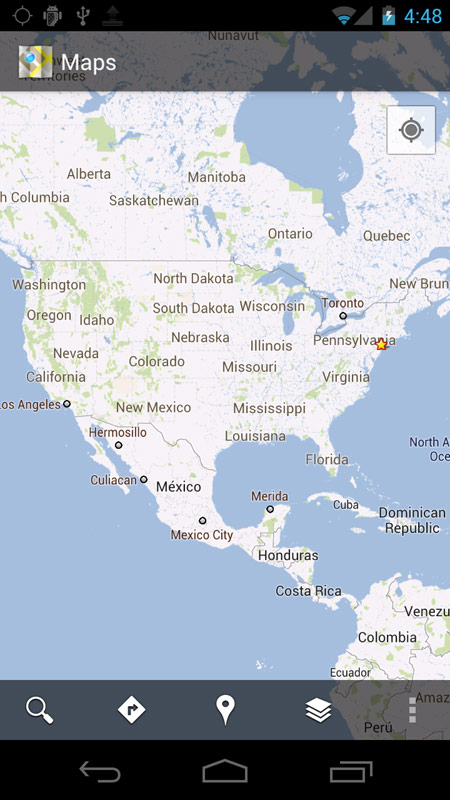
\includegraphics[scale=0.35]{map.jpg}
		\end{center}
	\item \textbf{Préférences} : Différents choix modifiant le comportement de l'application. \\
	La vue de présentation respectera le design et l'experience des menu classiques de préférences disponibles sur android avec cases à cocher ou autres widgets :
		\begin{center}
			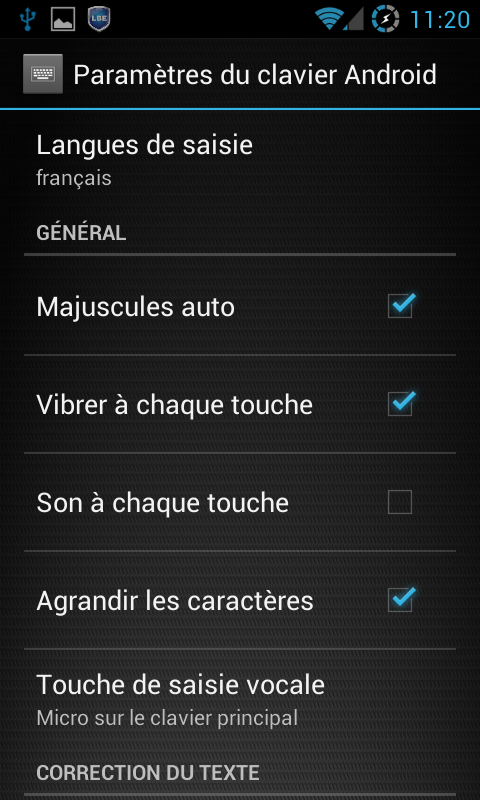
\includegraphics[scale=0.35]{preferences.png}
		\end{center}
	\item \textbf{Liste} : Choix lieu répertorié \\
	Cette vue permettra à l'utilisateur de parcourir l'ensemble des lieux répertoriés par l'application et éventuellement en choisir un.
	\end{itemize}
	
	\section{Réalisation}
	Dans cette section, nous allons présenter les différentes fonctionnalités que nous avons finalement développé pour cette application.
	
	\subsection{Application}
	% Carte
	\paragraph{Carte}
	Cette partie a été la première développée car c'est une fonctionnalité qui est à la base de toutes les autres. En effet, pour développer une application de guidage, l'affichage d'une carte est obligatoire. Soucieux de l'enjeu du logiciel libre, nous avons choisi de baser notre application sur \textit{OpenStreetMap} qui, de plus, est plus précise que \textit{Google Map} dans l'UM2. \\
	Afin que l'application soit accessible le plus rapidement possible, la carte est affiché dès le lancement de l'application : \\
	
	\begin{center}
		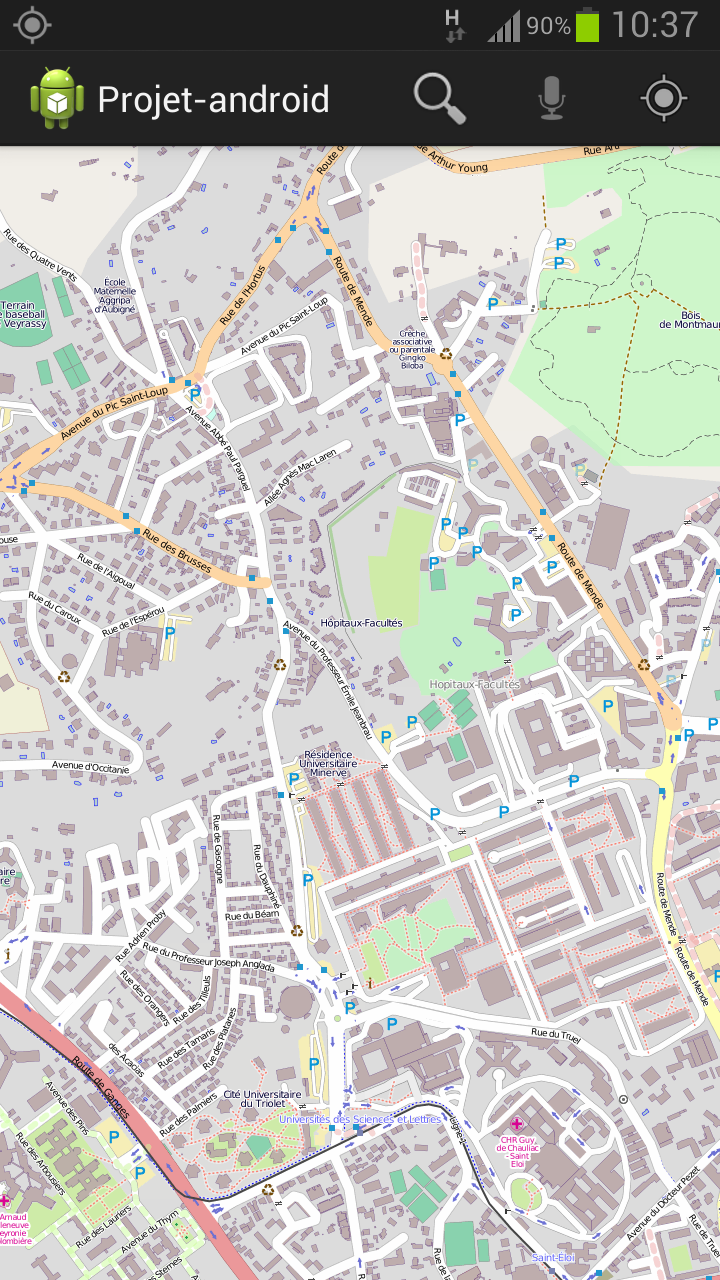
\includegraphics[scale=0.25]{carte.png}
	\end{center}
	
	% Recherche
	\paragraph{Recherche}
	Les deux premières icônes sur la barre d'outils servent à la recherche. La première ouvre la fenêtre de recherche textuelle. L'utilisateur peut alors rechercher un Bâtiment ou un point d'interêt. Si un lieu est trouvé, le chemin est tracé. Sinon, l'utilisateur est notifié du fait que rien n'a été trouvé. \\
	La deuxième correspond à la recherche vocale. Si l'utilisateur clique dessus, une fenêtre s'ouvre et il peut alors effectuer une recherche vocale. Par exemple, si on dit "Bâtiment 10" ou encore "Café" l'application va respectivement dessiner un chemin vers le Bâtiment 10, ou afficher l'emplacement des machines à café. \\
	
	\begin{center}
		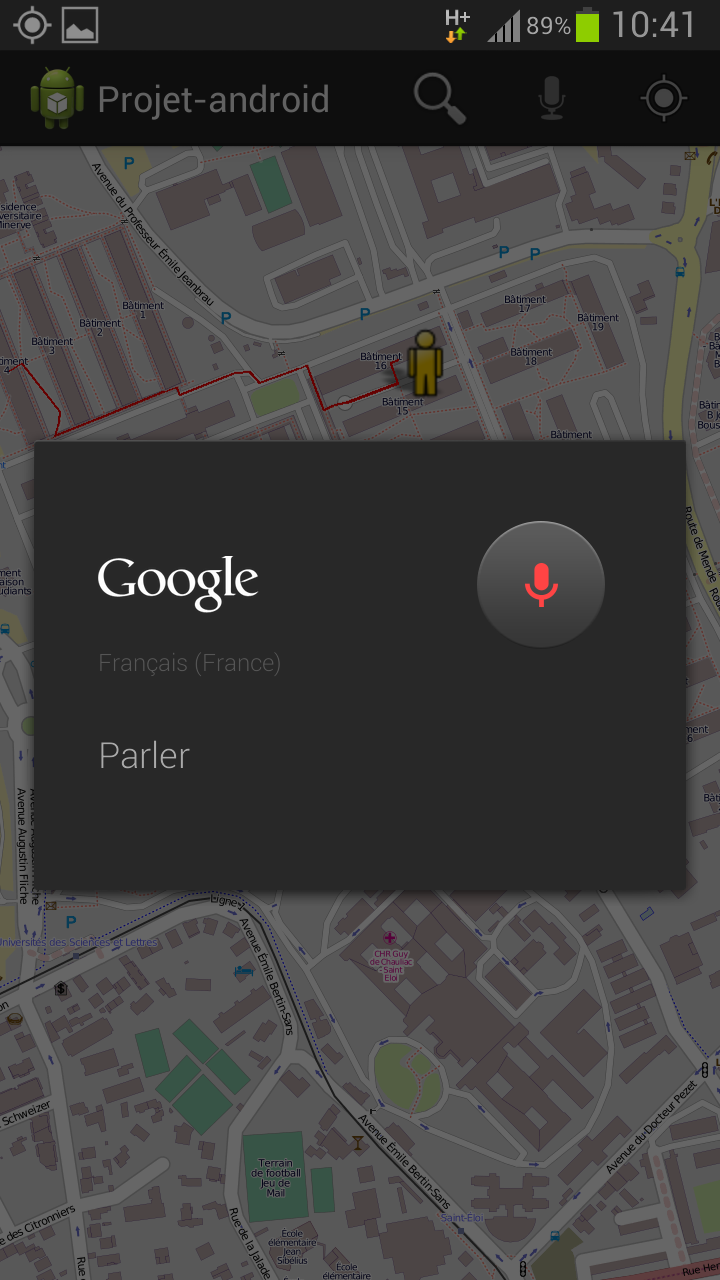
\includegraphics[scale=0.25]{recherche.png}
	\end{center}
	
	% GPS
	\paragraph{Guidage}
	L'application embarque un système de guidage de l'utilisateur. En effet, lorsque il recherche un Bâtiment ou qu'il en sélectionne un, le chemin le plus court est dessiné entre sa position et le lieu sélectionné. De plus, l'utilisateur peut choisir dans les préférences d'activer le guidage vocal à la manière d'un GPS classique. \\
	Enfin, l'utilisateur peut cliquer sur le troisième bouton de la barre d'outils qui permet de centrer la vue sur sa position. \\
	Pour tracer la route le guidage fait appel à une API REST : Yoursroute, une liste de points est retourné, et on dessine le chemin en rouge sur la carte en fonction. Cette API en appelle une autre pour avoir la description du chemin, pas exemple "tournez à gauche" etc.\\
	Le guidage vocal fonctionne assez simplement : YOURsroute retourne laliste des points de la route, et elle fait appel à une autre API pour avoir un descriptif dans la langue choisie (par exemple "Allez tout droit" puis "Tournez à droite").
	Il suffit ensuite de faire "lire" ce texte pour avoir un guidage vocal dans l'application. \\
	
	\begin{center}
   		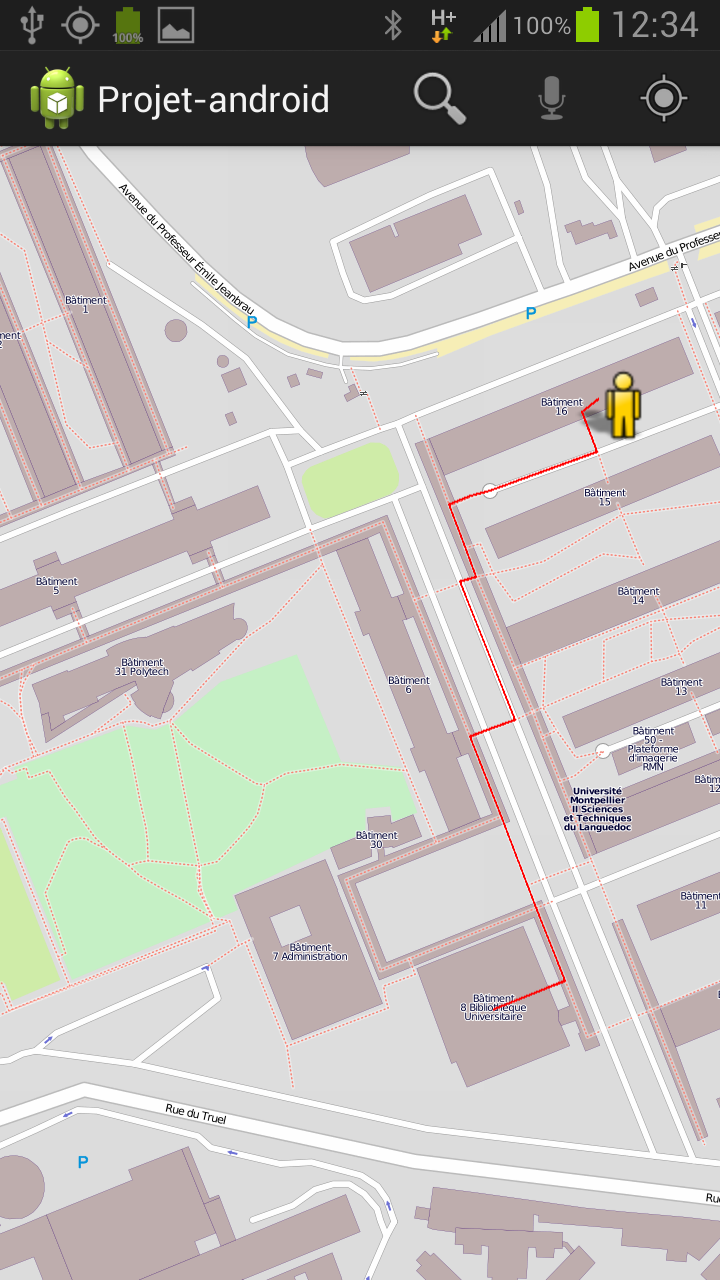
\includegraphics[scale=0.25]{guidage.png}
	\end{center}
	
	La recherche vocale utilise l'API de google, elle est assez permissive, par exemple la recherche reconnait "Bâtiment 16", "Bat 16", "16" ou encore par exemple "café" pour afficher la liste des machines à cafés dans la fac. \\
	De plus l'intégration du calendrier permet de rechercher (textuellement ou via la recherche vocale) "Prochain cours", ou encore "cours suivant". Si le mot est reconnu l'application effectue un guidage vers la salle du prochain cours de la journée.
	
	Il faut préciser que la recherche vocale et textuelle ont au final le même effet, car les chaînes de caractères sont traitées pareillement ensuite. C'est à dire que la recherche renvoie uniquement la chaîne reconnue et nous la traitons ensuite, il a fallu bien sûr rajouter quelques filtres pour considérer comme reconnues des expressions proches de celles recherchées. Pour café par exemple (symbolise les machines à café), nous acceptons le terme "ça fait". Ces résultats ont étés obtenus de manière empirique, c'est donc perfectible mais cela rend l'application plus tolérante lors d'une recherche vocale. \\
	% Liste
	\paragraph{Liste des lieux}
	Comme dit précédemment, l'utilisateur peut rechercher un Bâtiment pour se faire guider. De plus, en cliquant sur l'icône "lieux" de la barre d'outils, il obtient une vue à trois onglets : \\
	\begin{itemize}
		\item \textbf{Bâtiments} : Cet onglet affiche une liste des Bâtiments du campus Triolet. L'utilisateur peut cliquer dessus, et le guidage commence depuis sa position, vers le Bâtiment sélectionné.
		\item \textbf{Planning} : Depuis les préférences, l'utilisateur peut importer un fichier ".ics" contenant son emploi du temps (fichier exportable depuis ADT). Dans cette vue, la liste des cours de la journée s'affichent. L'utilisateur peut cliquer sur l'un d'entre eux, et le guidage commencera entre sa position et le Bâtiment ou a lieu le cours.
		\item \textbf{Autres} : Cet onglet affiche la liste des points d'intêrets de la fac. Il contient les points wifi, les machines à cafés, toilettes et parking.
		Si l'utilisateur clique dessus (par exemple café), des marqueurs vont s'afficher à chaque endroit où se trouve une machine à café. L'utilisateur n'aura plus qu'a faire un clic long sur l'un d'entre eux pour démarrer le guidage.
	\end{itemize}
	
	Pour afficher toutes ces informations, nous avons créé des fichiers csv, qui sont parsés avec une classe spécifique. Nous construisons ensuite des objets "Buiding". \\
	Ces informations sont ensuites toutes stockées en base de données via SQLite, et nous les retrouvons ensuite au besoin avec possibilité de filtrer les résultats. \\
	Pour le fichier ics, il est parsé grâce à la librairie iCal4j, nous avons redéfinies les classes d'évènements pour avoir uniquement les informations qui nous intéressaient et pouvoir les mettre facilement en Base de données. \\
	\begin{center}
		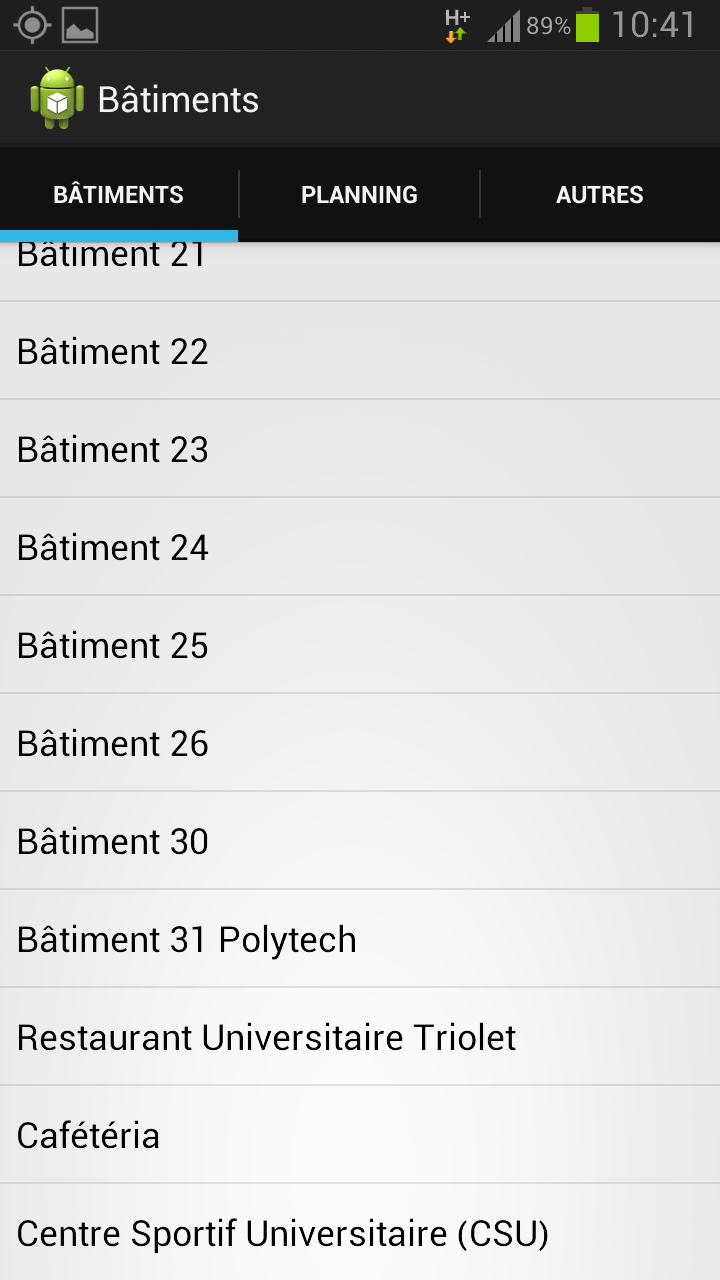
\includegraphics[scale=0.25]{liste.png}
	\end{center}
	
	Voici un screen de la liste des lieux avec les marqueurs sur la carte :
	\begin{center}
		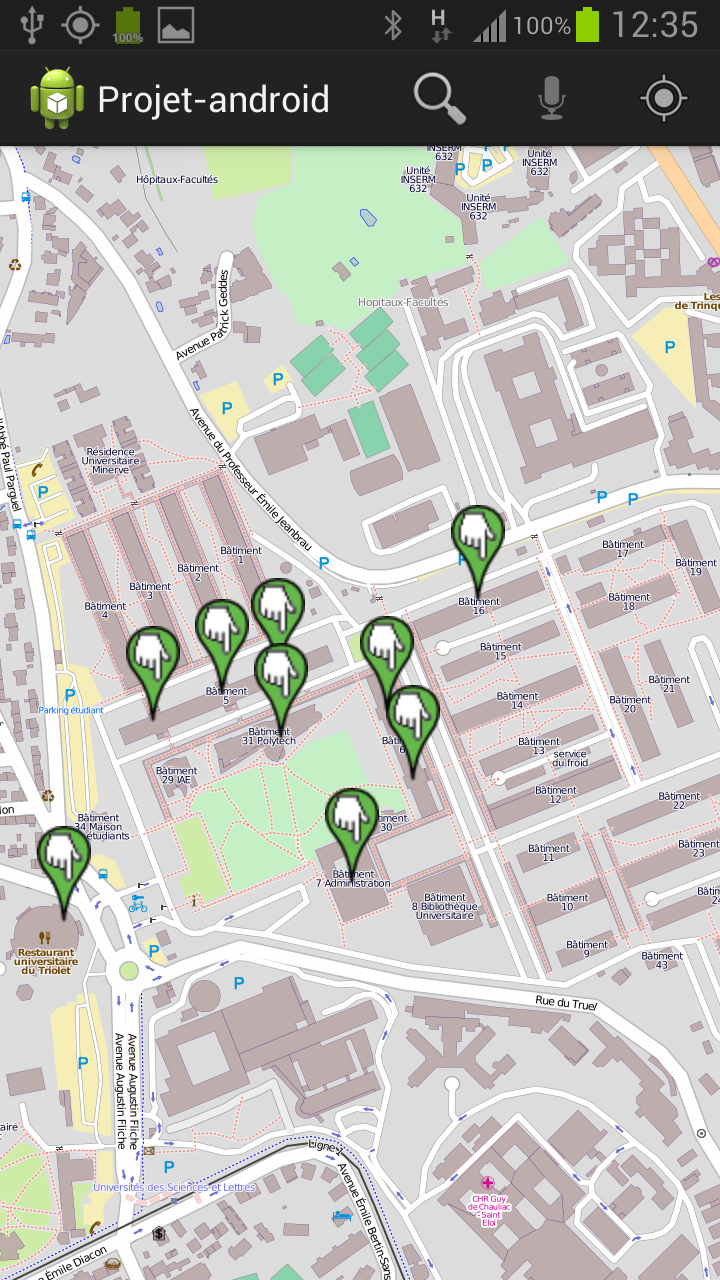
\includegraphics[scale=0.25]{marqueurs.png}
	\end{center}
	
	\subsection{Préférences}
	Pour permettre quelques réglages nous avons développés des préférences, il est donc possible d'activer ou non la guidage vocal. 
	De plus si on a rentré un fichier de calendrier, on peut activer le guidage automatique. C'est à dire que suivant l'heure l'application effectuera un guidage automatique vers le bâtiment du prochain cours. \\
	
	\begin{center}
		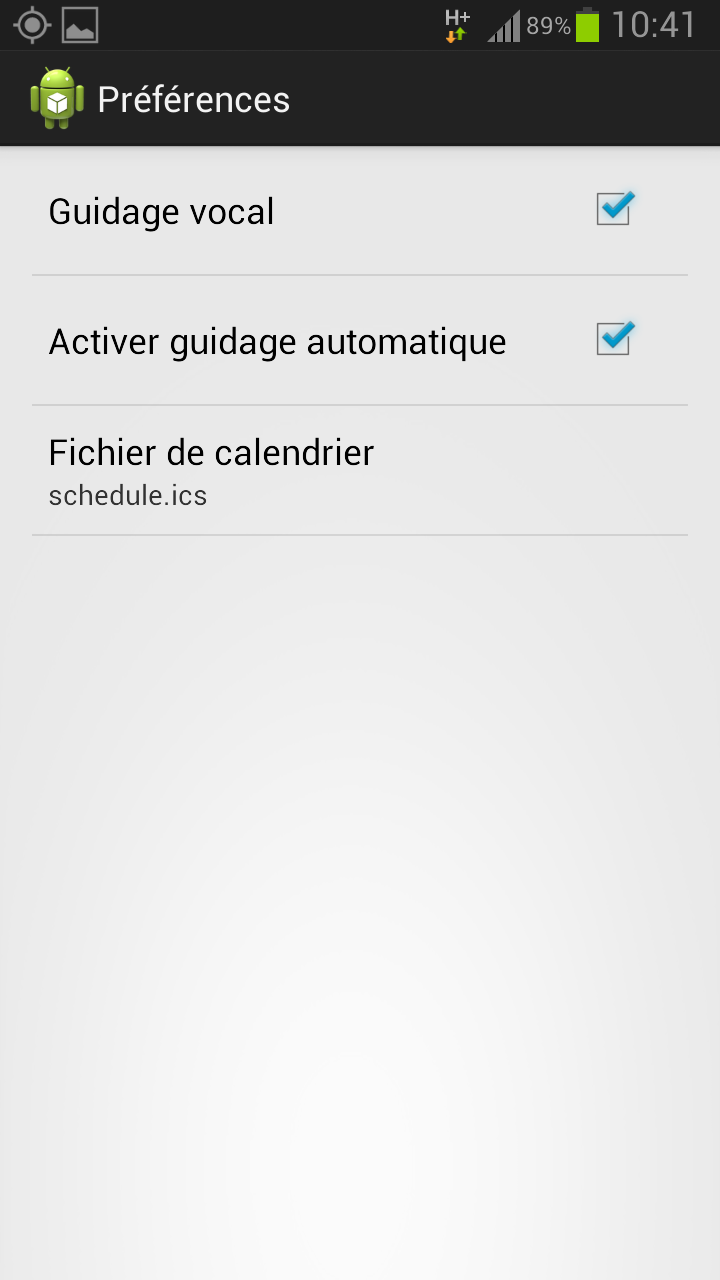
\includegraphics[scale=0.25]{reglages.png}
	\end{center}
	
	\subsection{Traduction}
	Dans l'optique de faire une application complète, nous l'avons traduite. \\
	En effet des étudiants étrangers peuvent être sur le campus, les menus et préférences sont donc traduits. Pour l'instant la seule langue disponible autre que le français est l'anglais, il faudrait idéalement plus de langues. \\
	La traduction utilise les mécanismes dédiés d'android, il y a donc toutes les chaînes traduites et l'application se base sur la locale du mobile pour définir la langue. \\
	
	\subsection{À propos}
	Il y a un petit menu à propos avec uniquement les noms des créateurs de l'application, on pourrait éventuellement rajouter la version de l'application. 
	
	\section{Conclusion}
		\subsection{Bilan}
		Nous avons donc une application avec les fonctionnalités présentes dans notre cahier des charges ainsi que des fonctionnalités souhaitées que nous avons pus finalement implémenter.
		L'application est traduite et possède assez d'informations de base pour être utilisable (et utile). \\
		
		\subsection{Difficultés}
		Une des difficultés rencontrée était les grands changements dans le SDK Android, il n'est pas rare de tomber sur des méthodes dépréciées, voir du code plus à jour ou qui ne marche plus sur internet. \\
		Nous avons trouvé la documentation pas toujours à jour, et pas forcément très claire. \\
		
		\subsection{Ouverture}
		Pour améliorer l'application il faudrait déjà plus de données, avec plus de points d'intêrets, on pourrait aussi traduire dans plus de langues.
		De plus il faudrait mieux gérer le cycle de vie de l'application, en particulier il faudrait arrêter tous calculs et affichage si l'application passe au second plan. \\
		Il faudrait également améliorer les cas spéciaux comme par exemple si on perd le GPS ou le réseau pendant l'utilisation. \\
		Une fonctionnalité manquante serait d'afficher la position courante même si il n'y a pas de destinations. \\
\end{document}
